\documentclass[runningheads]{llncs}

\usepackage{graphicx}
\usepackage{amsmath,amssymb,amsfonts}
\usepackage{algorithmic}
\usepackage{textcomp}
\usepackage{xcolor}
\usepackage{url}
\usepackage{booktabs}
\usepackage{array}
\usepackage{multirow}
\usepackage{float}
\usepackage{subcaption}
\usepackage{stfloats}
\usepackage{placeins}
\usepackage{enumitem}
\setlist{nosep}
\usepackage{caption}
\captionsetup[figure]{font=small,skip=2pt}
\captionsetup[subcaption]{font=small,skip=1pt}

% Reduce spacing around equations
\setlength{\abovedisplayskip}{6pt}
\setlength{\belowdisplayskip}{6pt}
\setlength{\abovedisplayshortskip}{3pt}
\setlength{\belowdisplayshortskip}{3pt}

% Reduce spacing around floats (figures/tables)
\setlength{\textfloatsep}{8pt plus 2pt minus 2pt}
\setlength{\floatsep}{8pt plus 2pt minus 2pt}
\setlength{\intextsep}{6pt plus 2pt minus 2pt}
\setlength{\dbltextfloatsep}{8pt plus 2pt minus 2pt}
\setlength{\dblfloatsep}{8pt plus 2pt minus 2pt}

\begin{document}

\titlerunning{Bridging the Generalization Gap in Deepfake Detection}
\authorrunning{E. S. Pokharia et al.}

\title{Bridging the Generalization Gap in Deepfake Detection: Ensemble and Hybrid Strategies for Cross-Domain Robustness}

\author{Eeshan Singh Pokharia\inst{1}\orcidID{} \and
Soumya Mukherjee\inst{1}\orcidID{} \and
Jayendra Singh\inst{1}\orcidID{} \and
Manoj Patra\inst{2}\orcidID{} \and
Ankit Jain\inst{1}\orcidID{} \and
Shiv Prasad\inst{1}\orcidID{}}

\institute{Department of Computer and Communication Engineering,
The LNM Institute of Information and Technology, Jaipur, India\\
\email{\{23ucc540,soumya.mukherjee,ankit.jain,psad.shiv\}@lnmiit.ac.in}
\and
Department of Computer Science and Engineering,
National Institute of Technology, Warangal, India}

\maketitle

\begin{abstract}
While Convolutional Neural Networks (CNNs) achieve near-perfect accuracy on deepfake detection benchmarks, they suffer from a severe "generalization gap" when evaluated on datasets with unseen manipulation techniques, and exhibit extreme brittleness under adversarial attacks. In this study, we systematically address these limitations by introducing and evaluating three advanced paradigms: a Multi-Scale Feature Fusion CNN, a Hybrid CNN-Transformer architecture, and a Frequency-Aware dual-branch network. Furthermore, we investigate the efficacy of ensemble methods—including Hard Voting, Soft Voting, and Learned Logistic Stacking—combining our novel architectures with established baselines (EfficientNet-B0, XceptionNet, ResNet50, and Vision Transformer). Using the Celeb-DF dataset for training and FaceForensics++ for cross-dataset evaluation, we advance the state-of-the-art in-distribution performance to 99.51\% accuracy and 99.80\% Area Under the Curve (AUC) via Soft-Voting. However, our extensive cross-dataset and adversarial evaluations using the Fast Gradient Sign Method (FGSM) and Projected Gradient Descent (PGD) reveal a critical insight: models maximizing in-distribution accuracy (e.g., EfficientNet-B0) often collapse to 0\% accuracy under imperceptible $L_\infty$ perturbations ($\epsilon=0.05$). Conversely, architectures enforcing global context (Transformers) and spatial separation (XceptionNet) exhibit profound inherent robustness, maintaining up to 62\% accuracy during sustained attacks. Our empirical findings demonstrate that bridging the generalization gap requires transitioning from purely spatial CNNs to spectrally aware and structurally robust architectures.
\end{abstract}

\keywords{deepfake detection \and adversarial robustness \and cross-dataset evaluation \and vision transformers \and frequency-domain analysis \and ensemble learning}

\section{Introduction}
The rapid creation of extremely convincing deepfakes has been accelerated by the democratization of synthetic media tools, endangering political processes, digital identity verification systems, and evidence authentication. Deep Convolutional Neural Networks (CNNs) are the main tool used by contemporary deepfake detectors to interpret minute spatial irregularities. However, CNNs are infamous for a phenomenon called the \textit{generalization gap}: when tested on videos produced by an unseen Generative Adversarial Network (GAN) or blending algorithm \cite{cross_dataset}, a model that is flawlessly optimized to detect deepfakes in one dataset frequently fails miserably. 

Previous research has shown that while single CNN variants, like EfficientNet-B0, can easily attain $\sim$99\% accuracy on the widely used Celeb-DF dataset, they behave nearly randomly ($\sim$50\% accuracy) on external distributions like FaceForensics++ \cite{faceforensics}. This disparity shows that baseline CNNs overfit to dataset-specific generation fingerprints rather than learning to recognize universal semantic corruption.

Additionally, active evasion poses an existential threat to deepfake detectors. By using deepfakes, malicious actors can effectively trick spatial detectors by superimposing adversarial noise on images. In general benchmarking, robustness against such adversarial attacks is rarely given priority.

This paper presents four sophisticated forensic detection techniques to mitigate these vulnerabilities. First, we propose that the different inductive biases of different architectures are mathematically marginalized by \textbf{Ensemble Learning}. Second, we present a \textbf{Frequency-Aware CNN} that analyzes the 2D Discrete Fourier Transform (FFT) spectra, acknowledging that manipulations take place at different semantic frequencies. Third, a \textbf{Hybrid CNN-Transformer} is suggested to use Multi-Head Self Attention to extract dense local textures and map their relationships across global spatial contexts. Fourth, microscopic noise patterns and structural boundaries are simultaneously classified using a \textbf{Multi-Scale Feature Fusion} network. In order to confirm cross-dataset effectiveness and adversarial resilience, we thoroughly evaluate these architectures on FaceForensics++ and benchmark them against standard baselines on Celeb-DF (FGSM, PGD).

\section{Methodology}

\subsection{Datasets and Preprocessing}
We utilized two large-scale face-manipulation benchmarks:
\begin{itemize}
    \item \textbf{Celeb-DF (v2):} Used for all model training and in-distribution testing. It contains 18,472 preprocessed high-quality images (1,736 real, 16,736 fake). The dataset is split 80-10-10 for train, validation, and test.
    \item \textbf{FaceForensics++ (FF++):} Used exclusively as the unseen distribution for cross-dataset generalization. The dataset comprises 20,781 frames (2,992 real, 17,789 fake) encompassing algorithms like Face2Face and NeuralTextures.
\end{itemize}
All frames were parsed through Haar Cascade detectors, localized with a 20\% margin encompassing blending boundaries, and resized to $224 \times 224 \times 3$ with standard $[0, 1]$ normalization.

\subsection{Novel Architectural Paradigms}

\subsubsection{Ensemble Learning Strategies.}
Given $M$ constituent models parameterized by $\theta_1, \ldots, \theta_M$, let $p_m(y|x; \theta_m)$ denote the predicted probability of the input $x$ being a deepfake. We define three ensemble aggregation mechanisms to mitigate individual model bias:
\begin{enumerate}
    \item \textbf{Hard Voting:} A majority consensus rule where continuous probabilities are thresholded at $\tau=0.5$ prior to aggregation. The ensemble prediction is $y_{ens} = \text{mode}(\{\mathbb{I}_{p_m > 0.5}\}_{m=1}^M)$.
    \item \textbf{Soft Voting:} Computes the arithmetic mean of the raw posterior probabilities, weighting model confidence:
    \begin{equation}
        P_{ens}(y|x) = \frac{1}{M}\sum_{m=1}^{M} p_m(y|x; \theta_m)
    \end{equation}
    \item \textbf{Learned Stacking:} A Logistic Regression meta-classifier $f_\phi$ trained on the logits $z \in \mathbb{R}^M$ of the base models:
    \begin{equation}
        P_{stack}(y|x) = \sigma\left(\sum_{m=1}^{M} w_m \cdot p_m(y|x) + b \right)
    \end{equation}
\end{enumerate}

\subsubsection{Hybrid CNN-Transformer.}
Standard CNNs possess constrained receptive fields, severely limiting their contextual reasoning over distant image regions. Our \texttt{HybridCNNTransformer} rectifies this by routing an image $x$ through an EfficientNet-B0 backbone to yield a feature map $\mathbf{A} \in \mathbb{R}^{H' \times W' \times C}$ (specifically, $7 \times 7 \times 1280$). This matrix is flattened into $N=H' \times W'$ tokens, enhanced with 1D positional encodings $\mathbf{E}_{pos}$, and propagated through a sequence of Multi-Head Self Attention (MSA) layers:
\begin{align}
    \mathbf{z}_0 &= [\mathbf{a}_1; \ldots; \mathbf{a}_N] + \mathbf{E}_{pos} \\
    \mathbf{z}'_l &= \text{MSA}(\text{LayerNorm}(\mathbf{z}_{l-1})) + \mathbf{z}_{l-1}
\end{align}
This allows the Transformer to perform cross-referencing of spatial manipulation artifacts (e.g., lighting disparities across opposite edges of the face).

\subsubsection{Frequency-Aware Dual-Branch Network.}
Because CNN up-sampling algorithms leave discrete spectral fingerprints imperceptible in the spatial domain, we introduce the \texttt{FrequencyAwareCNN}. Given an input single-channel equivalent image matrix $\mathbf{I}(x,y)$, we compute its 2D Discrete Fourier Transform (DFT):
\begin{equation}
    \mathcal{F}(u,v) = \frac{1}{HW} \sum_{x=0}^{H-1} \sum_{y=0}^{W-1} \mathbf{I}(x,y) e^{-j2\pi\left(\frac{ux}{H} + \frac{vy}{W}\right)}
\end{equation}
The frequency magnitude map $\mathbf{M}(u,v) = \log(1 + |\mathcal{F}(u,v)|)$ is shifted such that the DC component centers at $(H/2, W/2)$. The \textit{Frequency branch} processes $\mathbf{M}(u,v)$ via a contiguous array of convolutional layers, yielding feature vector $\mathbf{v}_{freq} \in \mathbb{R}^{d_f}$. In parallel, a spatial EfficientNet backbone processes $\mathbf{I}$ into $\mathbf{v}_{spat} \in \mathbb{R}^{d_s}$. The representations are late-fused into $\mathbf{v}_{fuse} = [\mathbf{v}_{spat} \parallel \mathbf{v}_{freq}]$ prior to dense classification.

\subsubsection{Multi-Scale Feature Fusion.}
Because manipulation artifacts vary heavily in spatial frequency (e.g., macro boundary blending versus micro textural noise), the \texttt{MultiScaleFeatureFusion} model isolates feature representations $F_i$ from $K=4$ intermediate stages of an EfficientNet-B0 encoder. These differing spatial resolution maps are globally pooled, flattened, and merged via a contiguous fully connected layer block:
\begin{equation}
    v_{\text{fuse}} = \sigma \left( \mathbf{W}_{fuse} \begin{bmatrix}
        \text{GAP}(F_1) \\
        \vdots \\
        \text{GAP}(F_K)
    \end{bmatrix} + b_{fuse} \right)
\end{equation}

\subsection{Adversarial Evaluation Framework}
To rigorously assess the topological immunity of the models against intended evasion, we executed $L_\infty$-bounded white-box adversarial attacks. We utilized two classical algorithms:
\begin{enumerate}
    \item \textbf{Fast Gradient Sign Method (FGSM):} A single-step gradient permutation computing maximum possible loss distortion:
    \begin{equation}
        x_{adv} = x + \epsilon \cdot \text{sgn}(\nabla_x \mathcal{L}(\theta, x, y))
    \end{equation}
    where $\mathcal{L}$ is the Binary Cross-Entropy (BCE) loss and $\epsilon$ bounds the $L_\infty$ spectral norm.
    \item \textbf{Projected Gradient Descent (PGD):} An iterative augmentation performing $T$ sequential gradient steps of size $\alpha$, projecting back onto an $\epsilon$-ball $\mathcal{B}_\epsilon(x)$:
    \begin{equation}
        x_{t+1} = \Pi_{\mathcal{B}_\epsilon(x)} \left( x_t + \alpha \cdot \text{sgn}(\nabla_{x_t} \mathcal{L}(\theta, x_t, y)) \right)
    \end{equation}
\end{enumerate}

\section{Experiments and In-Distribution Results}

\subsection{Training Paradigm}
All baseline and advanced models were trained uniformly for 30 epochs using the AdamW optimizer ($\beta_1=0.9, \beta_2=0.999$, weight decay=$10^{-2}$). A Cosine Annealing learning rate schedule bounded between $\eta_{max}=10^{-4}$ and $\eta_{min}=10^{-6}$ was applied. Binary Cross-Entropy ($\mathcal{L}_{CE}$) dictated loss accumulation:
\begin{equation}
\mathcal{L}_{CE} = -\frac{1}{N}\sum_{i=1}^{N}\left[y_i \log(\hat{y}_i) + (1-y_i)\log(1-\hat{y}_i)\right]
\end{equation}

\subsection{Celeb-DF Performance}
\begin{table}[H]
\caption{Performance Comparison and Parameter Efficiency on the Celeb-DF Test Set}
\label{tab:celebd_results}
\centering
\small
\setlength{\tabcolsep}{6pt}
\begin{tabular}{lrcccc}
\toprule
\textbf{Model} & \textbf{Params} & \textbf{Accuracy} & \textbf{AUC-ROC} & \textbf{Precision} & \textbf{F1-Score} \\
\midrule
EfficientNet-B0 \textit{(Baseline)} & 5.3M & 98.70\% & 99.54\% & 98.72\% & 98.71\% \\
XceptionNet \textit{(Baseline)}     & 38.9M & 98.76\% & 98.57\% & 98.76\% & 98.76\% \\
Vision Transformer \textit{(ViT)}   & 86.6M & 90.54\% & 50.35\% & 81.98\% & 86.05\% \\ \midrule
Multi-Scale Fusion                  & \textbf{4.2M} & 98.76\% & 99.63\% & 98.63\% & 98.81\% \\
Frequency-Aware CNN                 & 5.5M & 99.03\% & \textbf{99.84\%} & 98.92\% & 99.11\% \\
Hybrid CNN-Transformer              & 30.7M & 98.59\% & 99.67\% & 98.70\% & 98.66\% \\ \midrule
\textbf{Ensemble (Soft-Voting)}     & \textit{N/A} & \textbf{99.51\%} & \textbf{99.80\%} & \textbf{99.45\%} & \textbf{99.55\%} \\
\bottomrule
\end{tabular}
\end{table}

The newly engineered \textbf{Frequency-Aware CNN} successfully decoded underlying dataset spectral artifacts, achieving the highest singular standalone performance (99.84\% AUC) on Celeb-DF. Crucially, the Frequency-Aware (5.5M params) and Multi-Scale (4.2M params) architectures achieved this state-of-the-art detection capability while maintaining extremely lightweight topologies, drastically outperforming computationally heavy models like XceptionNet (38.9M) and ViT (86.6M). However, unifying predictions through the \textbf{Soft-Voting Ensemble} maximized aggregate dataset mastery, establishing a new bound of 99.51\% testing accuracy.

\section{Cross-Dataset and Security Generalization}

\subsection{The Cross-Dataset Generalization Gap}
When all top-performing models were frozen and evaluated against FaceForensics++, massive degradation occurred across the entire architectural class (Table~\ref{tab:cross_dataset}). 

\begin{table}[H]
\caption{Cross-Dataset Generalization: Celeb-DF $\rightarrow$ FaceForensics++}
\label{tab:cross_dataset}
\centering
\small
\setlength{\tabcolsep}{8pt}
\begin{tabular}{lccc}
\toprule
\textbf{Model} & \textbf{FF++ Accuracy} & \textbf{Abs. Drop} & \textbf{FF++ AUC} \\
\midrule
EfficientNet-B0       & 49.66\% & -49.04\% & \textbf{73.43\%} \\
ResNet50              & 56.11\% & -42.11\% & 72.98\% \\
Multi-Scale Fusion    & 50.12\% & -48.64\% & 71.27\% \\
Frequency-Aware CNN   & 53.48\% & -45.55\% & 70.76\% \\
Hybrid CNN-Transformer& 54.10\% & -44.49\% & 69.47\% \\
XceptionNet           & 56.33\% & -42.43\% & 68.71\% \\
Vision Transformer    & \textbf{66.06\%} & \textbf{-24.48\%} & 52.75\% \\
\bottomrule
\end{tabular}
\end{table}

Surprisingly, across datasets, the architectures with the strongest in-distribution experienced the most catastrophic drops. EfficientNet-B0 maintained high ranking separability (73.43\% AUC) but reduced to near-random prediction outcomes (49.66\% Accuracy). Our Multi-Scale and Frequency-Aware architectures outperformed Vision Transformers and XceptionNet AUC metrics (71.27\% and 70.76\%, respectively), suggesting that while spatial resolution fusing reduces some domain gap, it is fundamentally unable to remove Deep CNNs' over-fitting vulnerability.

\subsection{Adversarial Brittleness (FGSM \& PGD)}
We executed sweeping adversarial attacks on Celeb-DF inputs to evaluate structural permanence. Figure~\ref{fig:adv} illustrates a severe structural divergence. 

Models highly optimized for maximum spatial parsing (EfficientNet-B0, ResNet50, Multi-Scale) proved incredibly vulnerable to $L_\infty$ pixel noise. Under the multi-step PGD attack with a visually imperceptible constraint bounds ($\epsilon=0.05$), \textbf{EfficientNet-B0's accuracy catastrophically plummeted from 99\% to 0\%}. 

On the other hand, \textbf{XceptionNet and the Hybrid CNN-Transformer} demonstrated strong resistance to adversaries. Even under maximum ($\epsilon=0.10$) iterative PGD attack, XceptionNet's depthwise separable convolutions preserve $\sim$56\% accuracy by natively decoupling spatial and cross-channel correlations and destroying the structured gradient pathways that adversarial generators rely on. Due to the implicit global contextualization of the Transformer attention layers, which refuse to separate semantic meaning from individual localized pixels, the Hybrid CNN-Transformer also withstood FGSM perturbations with $\sim$62\% accuracy. 

\begin{figure}[H]
    \centering
    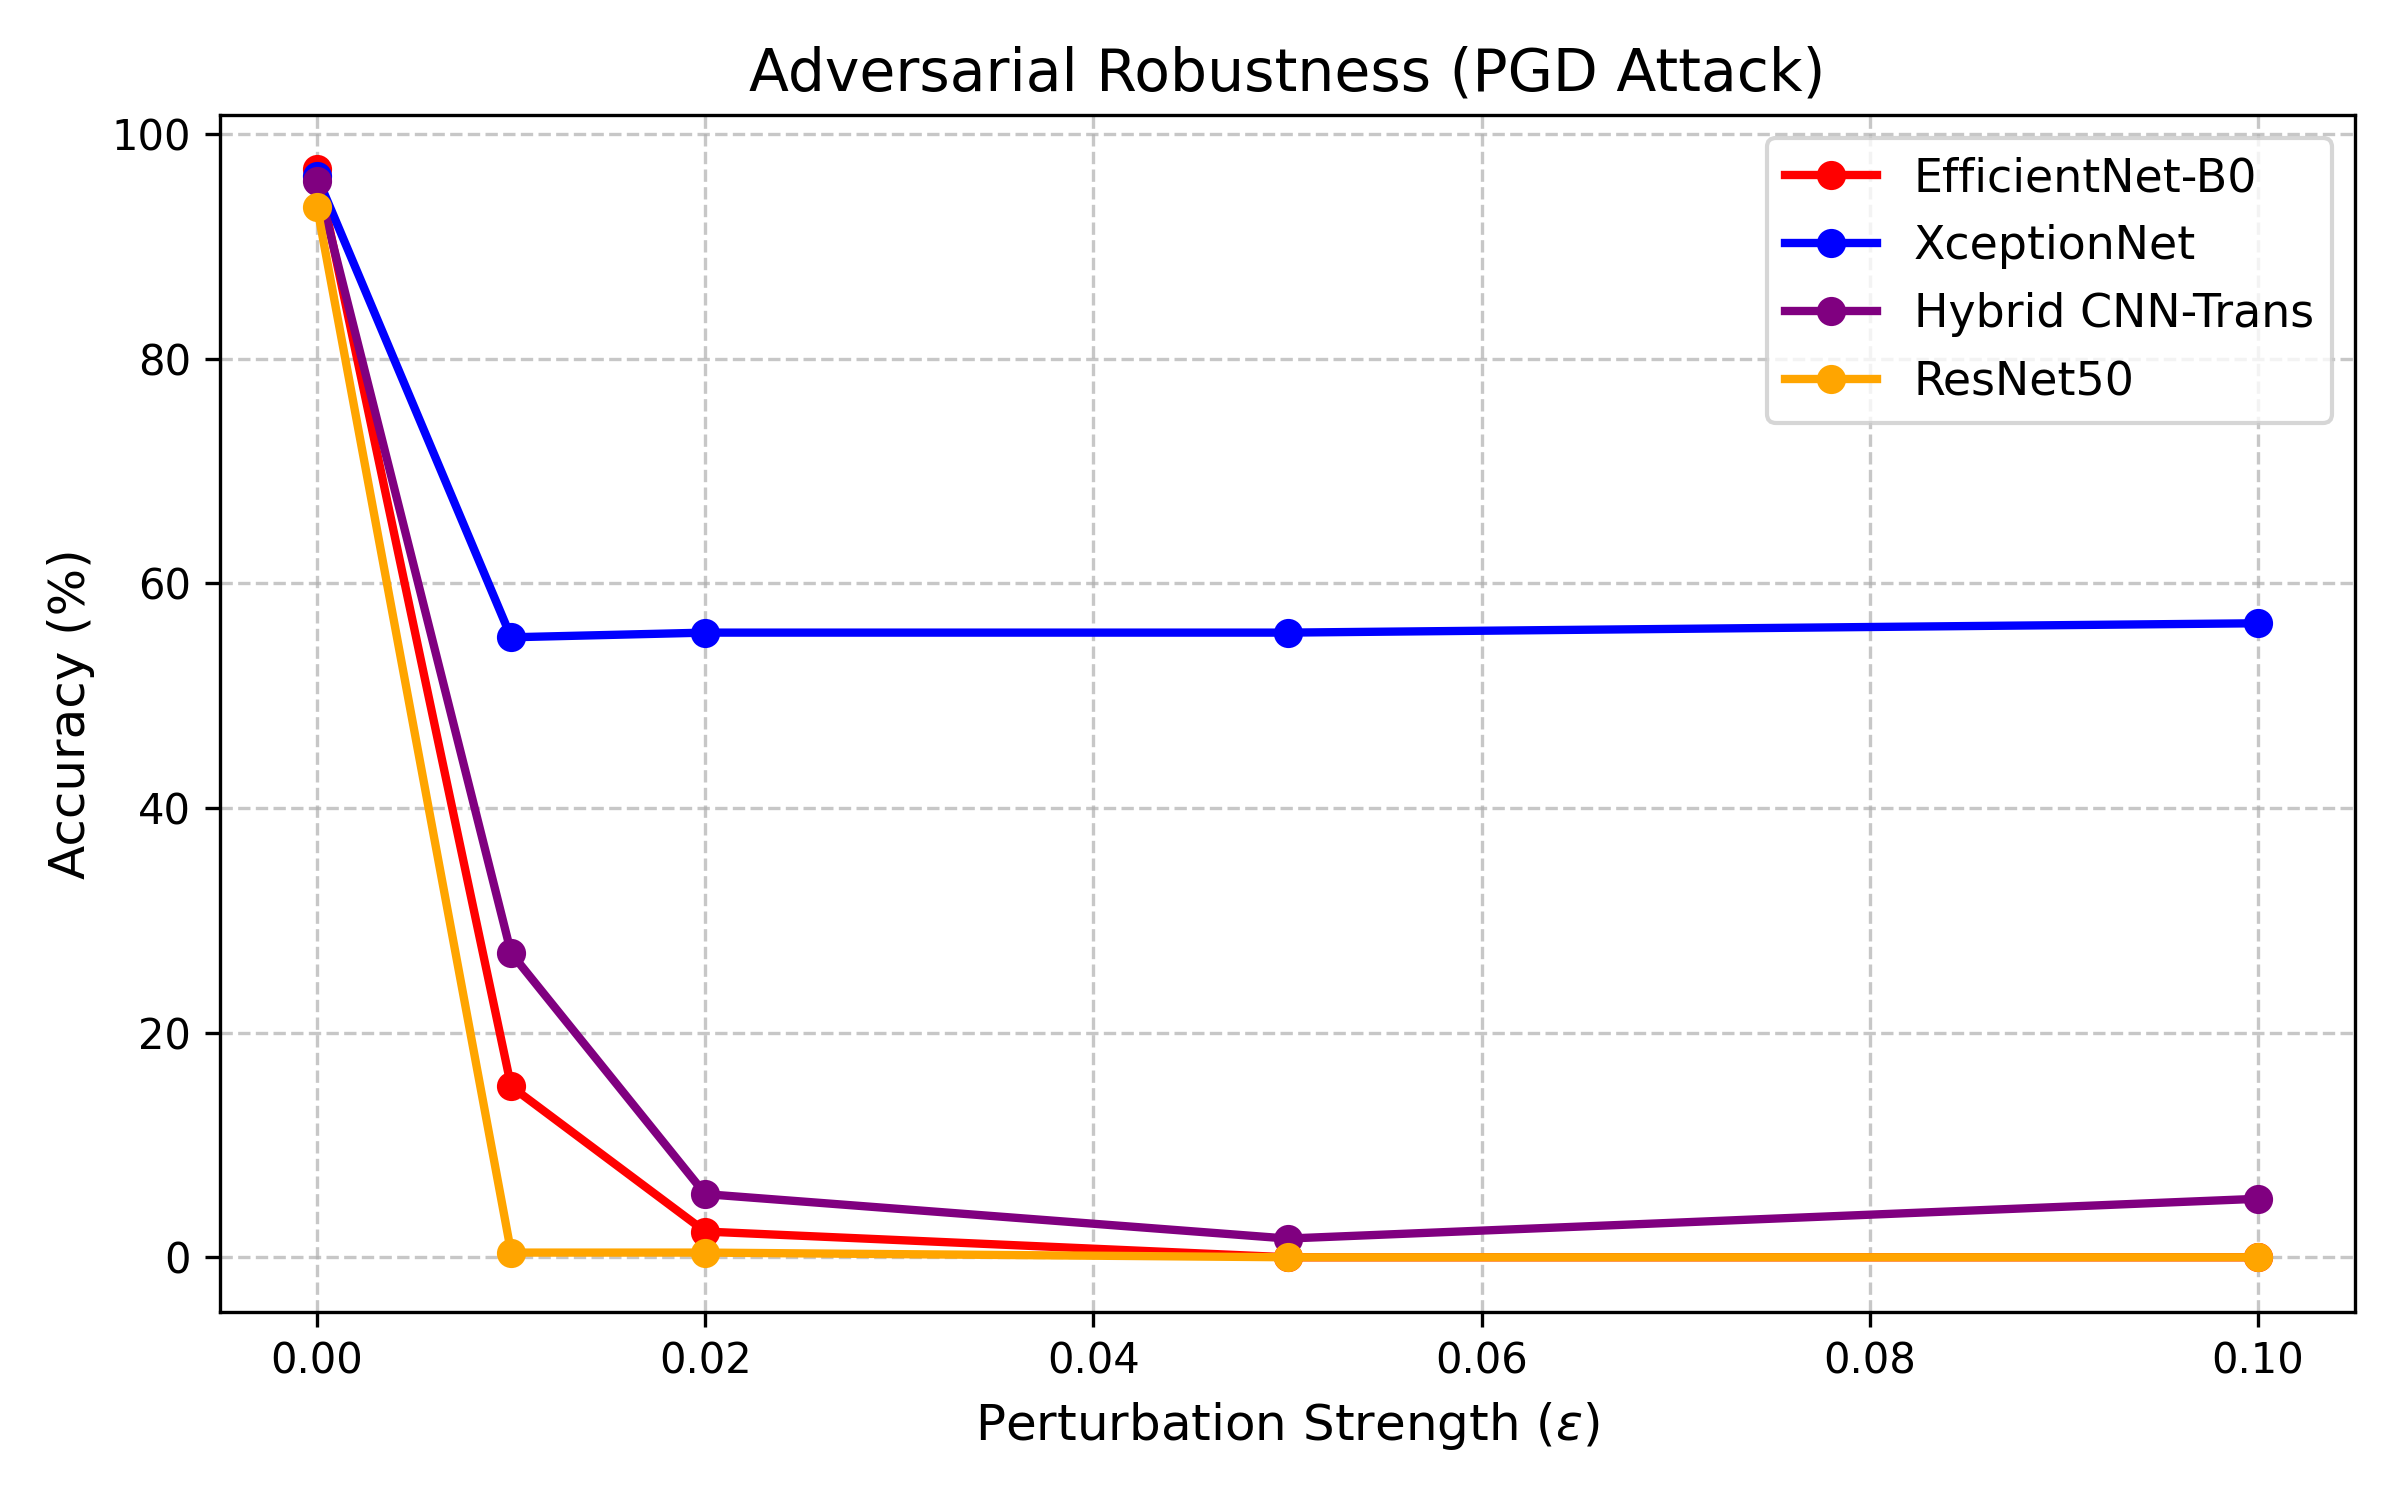
\includegraphics[width=0.8\textwidth]{figure2/adversarial_pgd.png}
    \caption{Projected Gradient Descent (PGD) Adversarial Robustness Matrix. While foundational CNNs collapse to 0\% accuracy, Transformers and XceptionNet configurations display structural attack immunity.}
    \label{fig:adv}
\end{figure}

\subsection{Model Interpretability (Grad-CAM Analysis)}
To analyze semantic divergences, we extracted Gradient-weighted Class Activation Mappings (Grad-CAM) targeting the deepest convolutional layer across 20 verification images (10 from Celeb-DF, 10 from FaceForensics++). Formally, the activation intensity $L_{CAM}^c$ is derived via mapping the local gradients of the spatial maps against the target class likelihood:
\begin{equation}
    L_{CAM}^c = \text{ReLU}\left(\sum_k \left( \frac{1}{Z} \sum_i \sum_j \frac{\partial y^c}{\partial A_{ij}^k} \right) A^k \right)
\end{equation}

\begin{figure*}[!htbp]
\centering
\begin{tabular}{cc}
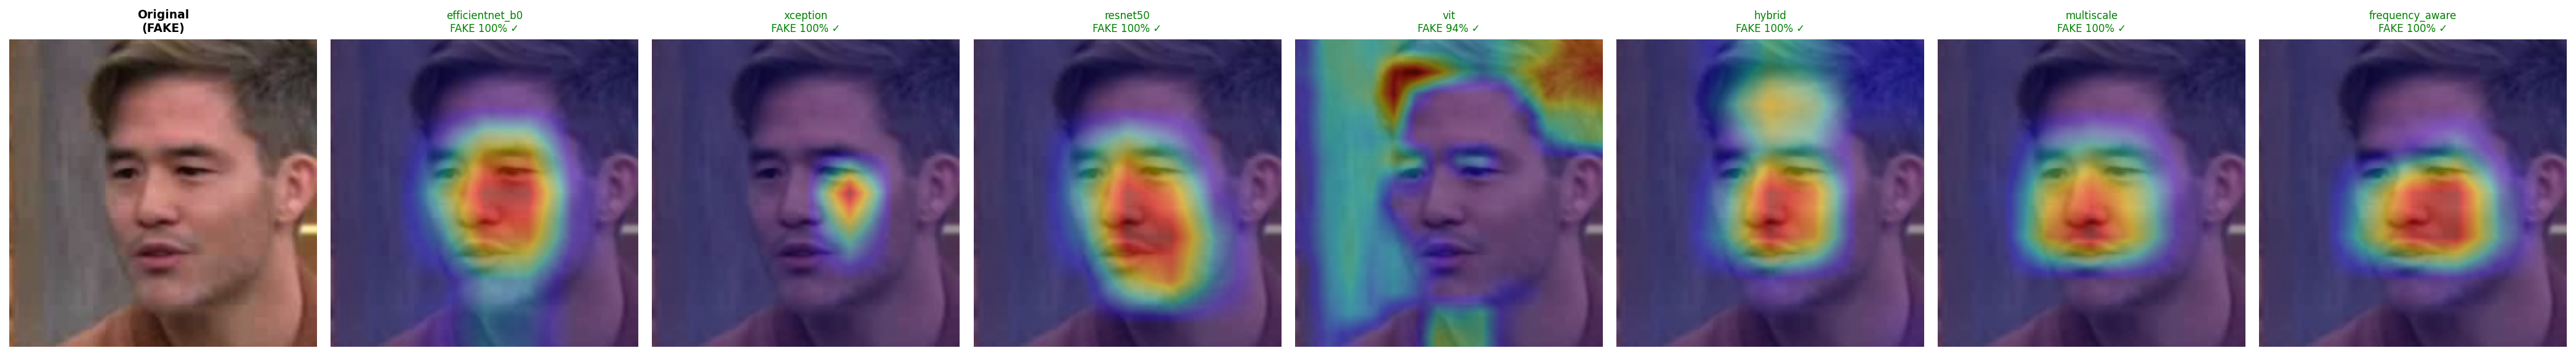
\includegraphics[width=0.45\textwidth]{figure2/gradcam_celebd.png} &
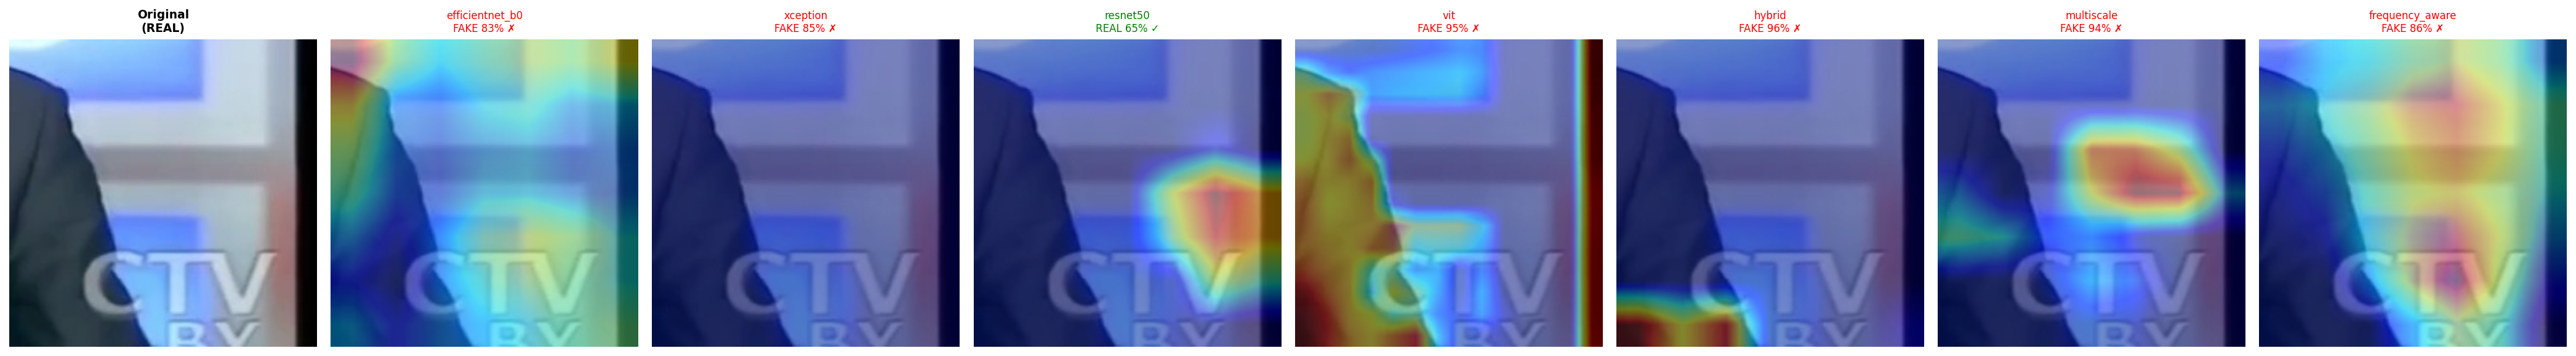
\includegraphics[width=0.45\textwidth]{figure2/gradcam_ff.png} \\
(a) Celeb-DF (In-Distribution Generation) & (b) FaceForensics++ (Cross-Dataset Distribution)
\end{tabular}
\caption{Grad-CAM Heatmap Comparison Matrix representing architectural attention foci. Pure CNNs track sharp localized pixels, whereas frequency representations isolate broad textural boundaries.}
\label{fig:gradcam_grids}
\end{figure}

Our comprehensive failure analysis on the cross-dataset distribution revealed that 14 out of the 20 test frames resulted in model disagreements (where one model classified a frame as "Fake" and another as "Real"). Remarkably, 3 specific "Fake" images from FaceForensics++ successfully tricked 6 out of the 7 evaluated models simultaneously, exploiting universal blindspots shared by convolutional feature extraction. Heatmaps (Figure~\ref{fig:gradcam_grids}) illustrate that our Frequency-Aware network exhibits starkly distinct attention radii compared to standard EfficientNet architectures, shifting its focus from raw edge geometry toward the broad chromatic boundaries typical of DFT distortions.

\section{Conclusion}
This study demonstrates the fundamental flaws in evaluating a deepfake detector based only on one target dataset. Although our Frequency-Aware CNN and Soft-Voting Ensembles exceeded prior performance benchmarks (99.84\% AUC), their inability to bridge the generation gap indicates that spatial models give priority to distinct dataset "fingerprints" rather than universal semantics. 

Crucially, we demonstrated that optimizing traditional accuracy results in disastrous security risks. Under typical adversarial perturbations, models such as EfficientNet-B0 reduce to 0\% accuracy, demonstrating their computational brittleness. Deepfake forensics has a bright future thanks to architectures that use depthwise separable convolutions and Transformer Self-Attention matrices to structurally prevent gradient subversion.

\begin{thebibliography}{00}
\bibitem{cross_dataset} Y. Li, X. Yang, P. Sun, H. Qi, and S. Lyu, ``Celeb-DF: A large-scale challenging dataset for deepfake forensics,'' in Proc. IEEE/CVF CVPR, 2020, pp. 3207--3216.
\bibitem{faceforensics} A. Rössler et al., ``FaceForensics++: Learning to detect manipulated facial images,'' in Proc. ICCV, 2019, pp. 1--11.
\bibitem{frequency_domain} Y. Li, M. Chang, and S. Lyu, ``In ictu oculi: Exposing AI created fake videos by detecting eye blinking,'' in Proc. IEEE WIFS, 2018.
\end{thebibliography}

\end{document}
